\chapter{Result}
This chapter presents the results from the conducted evaluation. Appendix \ref{appendix:raw} contains raw data and metrics over data that may not been presented in this chapter. The chapter start which presenting the results from the \textit{\nameref{Performance}} evaluations where the parameters time and memory is measured. Next and last section is \textit{\nameref{Applications}} where Java applications have been evaluated measuring security vulnerabilities with and without Dynamic Taint Propagation.



\section{Performance Overhead}
\label{Performance}
The results from benchmarking the application on DaCapo Benchmark Suit \parencite{dacapo} is seen in Figure \ref{fig:Time} and \ref{fig:Memory}. Both graphs are constructed to show the added overhead of running the applications with Dynamic Taint Tracking activated. The graphs are conducted based on the data in Table \ref{TimeTable} and \ref{MemoryTable}.



\subsection{Time}
Figure \ref{fig:Time} displays the results of the average time overhead per application. The results show that the application with the least average time overhead was Tradesoap where 14.7\% was added. The largest application however, was Fop with an overhead of 426.2\%. The average overall is 142.1\%.

\begin{figure}[!hbt]
	\centering
	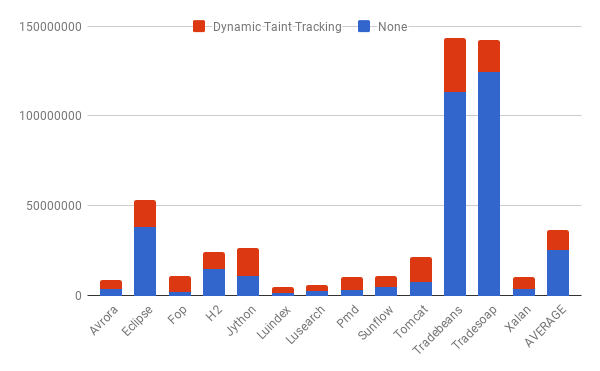
\includegraphics[width=\textwidth]{images/Time.png}
	\caption{Average Added Time in Microseconds}
	\label{fig:Time}
\end{figure}



\subsection{Memory}
Figure \ref{fig:Memory} displays the results of the average memory overhead per application. The results show that the application with the least average memory overhead was Eclipse where 5.5\% was added. The largest application however, was Fop with an overhead of 277.8\%. The average overall is 127.2\%.

\begin{figure}[!hbt]
	\centering
	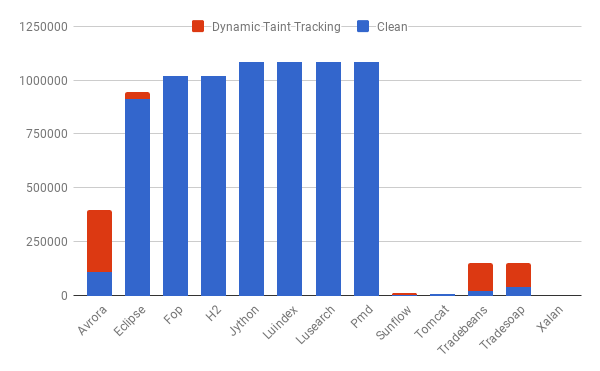
\includegraphics[width=\textwidth]{images/Memory.png}
	\caption{Average Added Memory in Kilobytes}
	\label{fig:Memory}
\end{figure}



\section{Applications}
\label{Applications}
The presented results in this chapter are from evaluating Java applications for security vulnerabilities with and without Dynamic Taint Tracking. The results from each application is listed in its own table where vulnerability type and number of vulnerabilities is listed. In the presentation of the result in text are vulnerabilities of the same type aggregated.

Table \ref{table:MicroTable} shows the vulnerabilities from evaluating Stanford SecuriBench Micro \parencite{securiBenchMicro}. In the table can we see that the most frequent vulnerability is reflected XSS where 71 vulnerabilities are present. Second most common is SQL Injection with 20 and the least common with 1 vulnerability is Buffer Overflow. By enabling Dynamic Taint Tracking on the Stanford SecuriBench Micro \parencite{securiBenchMicro} application results in a 100\% prevention rate.

\begin{table}[!hbt]
  \centering
  \caption{Security Vulnerabilities Found in Stanford SecuriBench Micro}
  \label{table:MicroTable}
    \begin{tabular}{rcc}
      & \textbf{None} & \textbf{Dynamic Taint Tracking} \\
      \textbf{Cross Site Scripting (Reflected)} & 71            & 0  \\
      \textbf{SQL Injection}                    & 20            & 0  \\
      \textbf{Buffer Overflow}                  & 1             & 0  
    \end{tabular}
\end{table}

Table \ref{table:InsecureTable} shows the vulnerabilities from running Insecure \parencite{insecure} with and without Dynamic Taint Tracker. Of the two types of vulnerabilities is SQL Injection the first with six vulnerabilities abd reflected XSS with two. Enabling Dynamic Taint Tracking on Insecure \parencite{insecure} results in 100\% prevention rate on SQL Injection attacks and 0\% for XSS. The overall prevention rate is 75\%. 

\begin{table}[!hbt]
  \centering
  \caption{Security Vulnerabilities Found in Insecure}
  \label{table:InsecureTable}
    \begin{tabular}{rcc}
      & \textbf{None} & \textbf{Dynamic Taint Tracking} \\
      \textbf{Cross Site Scripting (Reflected)}      & 2             & 2  \\
      \textbf{SQL Injection - Authentication Bypass} & 2             & 0  \\
      \textbf{SQL Injection - Hypersonic SQL}        & 4             & 0  
    \end{tabular}
\end{table}

The results from evaluating the application SnipSnap \parencite{snipsnap} is seen in Table \ref{table:SnipSnapTable}. In this table can we see that the most common vulnerability is reflected XSS with 172 occurrences. Second Largest is SQL Injection with 49 occurrences followed by CRLF Injection with two. Enabling Dynamic Taint Tracking yields in a overall prevention rate of 77.2\%. All CRLF Injection are prevented. XSS is prevented to 77.3\% and SQL Injection with 75.5\%.

\begin{table}[!hbt]
  \centering
  \caption{Security Vulnerabilities Found in SnipSnap}
  \label{table:SnipSnapTable}
  \begin{tabular}{rcc}
    & \textbf{None} & \textbf{Dynamic Taint Tracking} \\
    \textbf{Cross Site Scripting (Reflected)}      & 172           & 39   \\
    \textbf{CRLF Injection}                        & 3             & 0    \\
    \textbf{SQL Injection}                         & 47            & 10   \\
    \textbf{SQL Injection - Authentication Bypass} & 2             & 2       
  \end{tabular}
\end{table}

Table \ref{table:Ticketbook} shows the vulnerabilities from evaluating Ticketbook \parencite{ticketbook}. The most common vulnerability was XSS with 14 occurrences. SQL Injection was the least with one. The prevention rate of SQL Injection was 100\% and for XSS 71.4\%. The overall prevention rate is 73.3\%.

\begin{table}[!hbt]
  \centering
  \caption{Security Vulnerabilities Found in Ticketbook}
  \label{table:Ticketbook}
  \begin{tabular}{ccc}
    & \textbf{None} & \textbf{Dynamic Taint Tracking} \\
    \textbf{Cross Site Scripting (Persistent)} & 2             & 0 \\
    \textbf{Cross Site Scripting (Reflected)}  & 12            & 4 \\
    \textbf{SQL Injection}                     & 1             & 0
  \end{tabular}
\end{table}